\documentclass[dvips,letterpaper,12pt]{report}
\usepackage{thesis}
\usepackage{natbib}

\begin{document}

\pagenumbering{roman}

% Fill in the title, author, degree name, department, and month/year.
% Upon completion, this should look like the following:
%\thesistitle
%	{Complicated and Important-Sounding Thesis Title}
%	{John P. Doe}
%	{Master of Science}
%	{Department of Computer Science}
%	{May 2009}
% The \thesistitle definition is in thesis.sty.  Other customizations
% can be made there.
\thesistitle
	{Metathesis: \\
	 A \LaTeX\ template to Typeset Your Thesis for \\
	 Submission to the School of Graduate Studies  \\
	 \footnotesize{\sl (Changed the title by modifying the file
	  \texttt{thesis.tex})}}
	{\emph{my-name} (change this in \texttt{thesis.tex})}
	{Master of \emph{faculty} \textbf{or} Doctor of Philosophy
	 (change this in \texttt{thesis.tex})}
	{Department of \emph{dept-name}
	 (change this in \texttt{thesis.tex})}
	{\emph{Month Year} (change this in \texttt{thesis.tex}, too)}

\addcontentsline{toc}{chapter}{Abstract}



\begin{center}
\textbf{\large Abstract}
\end{center}


\emph{``High intensity focused ultrasound treatment is a potential non-invasive treatment which uses ultrasound energy generated by a piezoelectric (ferroelectric) transducer to thermally ablate tumour tissues. However, the issue that is preventing the treatment from being more widely available is a prominent treatment cost in comparison to alternative therapies. The high treatment cost can be attributed to the longer operation time with cycles of heating and cooling. This heating and cooling cycle is applied in order to prevent overheating of the ferroelectric material which is used to generate the ultrasound. Overheating of the transducer can change the effective thickness frequency relationship of the material and can even lead to depolarization of the material. The overheating is caused by the energy loss (dielectric dissipation), which occurs when the alternating electric field is applied and converted into the ultrasound. The associated material characteristics are the quality factor or tan , which is a macroscopic property. Alternatively, the loss can also be related to the area of the hysteresis loop of the particular material. This project aims at searching for potential ferroelectric materials with reduced overheating which in turn means a material with reduced hysteresis area (or low tan ). At the initial stage, first principle approaches have been adapted in our research rather than experimental methods, which would consume more effort in terms of equipment, capital and time.  For the purpose of study, all electron density functional package �WIEN2k� with the help of high performance computing is being used. In order to determine the ferroelectric parameters which are related to the polarization based property of materials, an additional software �BerryPI� has been developed in the framework of our research. The property of interest (tan? or hysteresis area) which is measured at macroscopic level has been brought down to microscopic level where it has been related to the barrier height of the potential curve of the ferroelectric materials. Based on this relation our plan is to perform screening of potential ferroelectric materials aiming at optimizing the produced mechanical energy to power loss ratio.''}


\addcontentsline{toc}{chapter}{Acknowledgements}
\begin{center}
\textbf{\large Acknowledgements}
\end{center}


\tableofcontents

\addcontentsline{toc}{chapter}{List of Tables}
\listoftables

\addcontentsline{toc}{chapter}{List of Figures}
\listoffigures


\pagenumbering{arabic}
\chapter{Introduction}
\label{chap:intro}


\section{Introduction to High Intensity Focused Ultrasound (HIFU)}

When one thinks of tumor surgery the things that come to mind are an operative room, lots of instruments to incise the body with surgeons holding them and finally a long recovery time where the affected patient has  to stay in special care for weeks, months or may be more. Such a treatment causes pre operative fear in patient's mind~\cite{Ramsay.1972.A.396}. Such pre-operative fear can in turns results in long recovery time, negative emotions and in some cases it forces the patient to use analgesics ~\cite{Sime1976}. These factors inspires people to develop an ideal tumor surgery which will avoid the above complications. An ideal tumor surgery would be a treatment which would require no incision and as a result shorter recovery time of the patient can be achieved This should be able to remove the affected tissue without damaging the adjacent structures near that tissue ~\cite{Jolesz...1}. The non-invasive nature of the treatment would be able change existing clinical practises and make it more patient friendly.
\begin{figure}[t]
\centering
	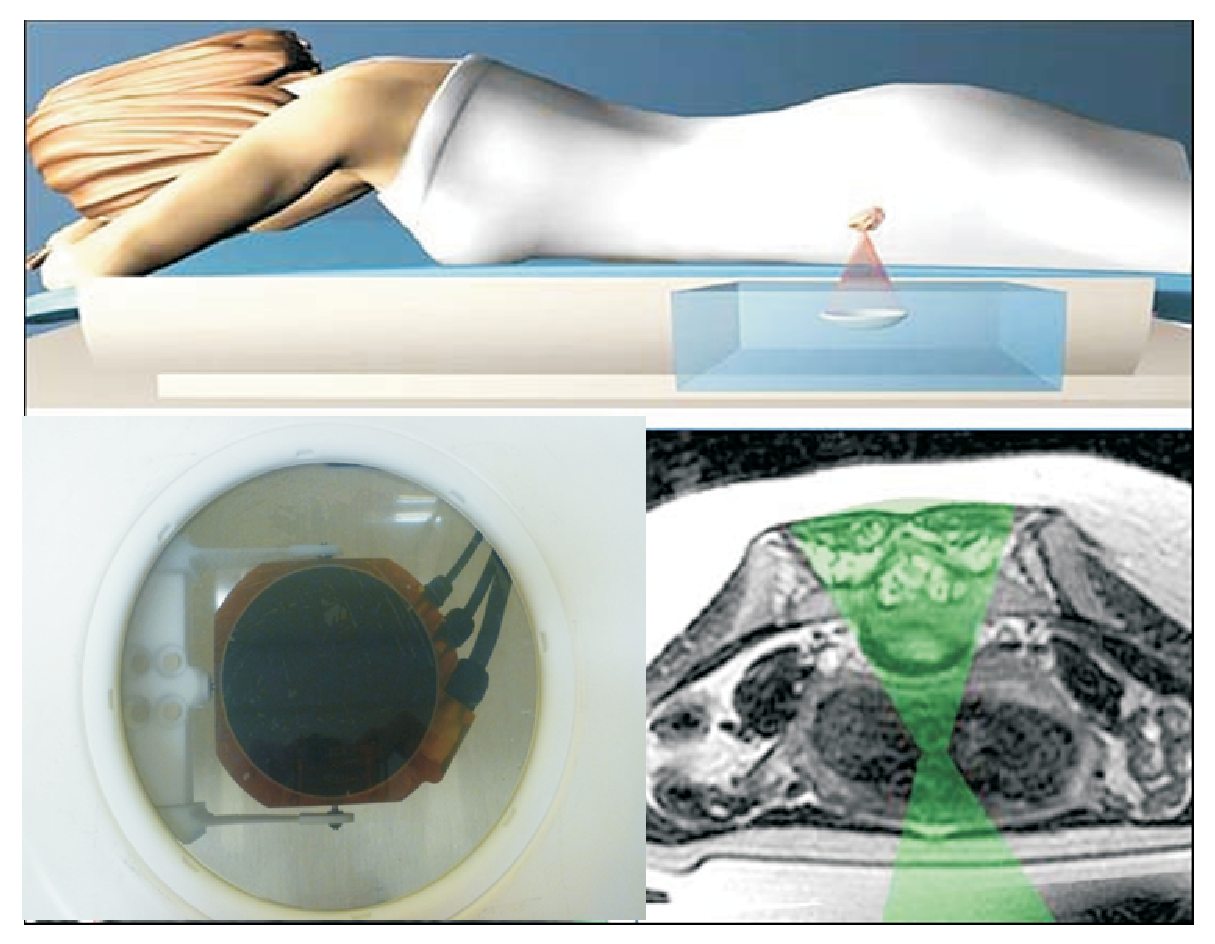
\includegraphics[width=0.7\textwidth]{Ultrasounf_focused.eps}\\
	\caption[Focusing of ultrasound]{Focusing of ultrasound\footnote}\label{fig:Ultrasounf_focused}

\end{figure}
\footnotetext{http://brainchemist.wordpress.com/2010/11/09/mri-guided-focused-ultrasound-surgery-radiology-brigham-and-womens-hospital-harvard}

Magnetic resonance guided high intensity focused ultrasound treatment(MRgFUS) is considered to be a potential candidate for such an ideal tumor surgery ~\cite{Jolesz...1}. In this treatment Magnetic resonance imaging (MRI) is used to localized the target tumor. Then an ultrasound energy is generated by vibrating a piezoelectric materials and focused on the target tumor tissue (Figure~\ref{fig:Ultrasounf_focused}). The acoustic energy because of its unique nature just focused at the particular tumor tissue. Upon focusing the acoustic energy is converted into heat and thus thermally coagulate the tissue. The energy deposition doesn't cause any bio-effects to the adjacent healthy tissues or even tissues and skin on its path to the tumor tissue. The thermal ablation process require controlled monitoring in order to prevent overheating of tissues. MRI also has capability of mapping temporal and spatial distribution of tissues. This MRI feature is utilized to monitor the thermal ablation process..

\begin{figure}[t]
\centering
	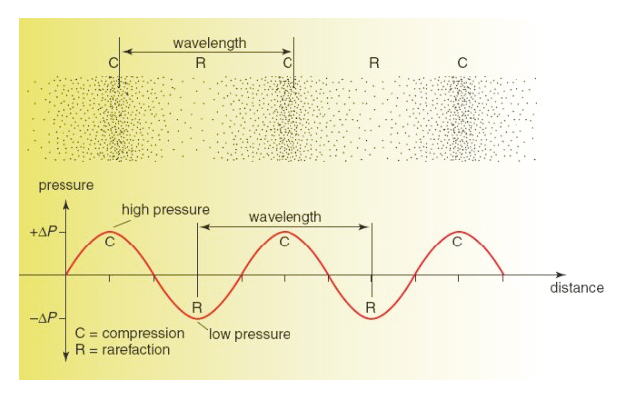
\includegraphics[width=0.7\textwidth]{Compressionandrarefactioncollected.eps}\\
	\caption[Compression and rarefaction of sound wave]{Compression and rarefaction of sound wave\footnote}\label{fig:Compression and rarefaction}
\end{figure}
\footnotetext{http://www.genesis.net.au/~ajs/projects/medical\_physics/ultrasound/index.html}


\section{Basic Principle}

\subsection{Ultrasound Generation}
Ultrasound are basically sound waves with frequency greater than 1MHz. As human ear audible range is 20 Hz to 20000 KHz, it can't be heard by human being.Unlike other sound wave ultrasound propagate in a medium through vibration of molecules.First sound is generated from a source which initiate vibration. The vibration is transferred inside the medium to neighboring molecules. As a result compression and rarefaction takes place(Figure~\ref{fig:Compression and rarefaction}) where compression refers to the situation when molecules are pressed together or forced and rarefaction refers to the situation when the molecules are weakly bound or free to move.Moleculer vibration can take place in both longitudinal (longitudinal wave) and transverse(shear wave) direction. For medical ultrasound purposes shear wave is not used as it gets attenuated quickly is soft tissues~\cite{Hynynen...5,Carson.1978.JCU.126,Hunt.1987..354,Hynynen.1990..61}.




\subsection{Ultrasound Transducer}
Transducer is a device that converts one form of energy into another.Ultrasonic transducer is also one form of energy conversion device which converts electrical energy into mechanical energy using the piezoelectric effect.The transducer is operated at the resonance frequency of the piezoelectric material where it present higher response~\cite{Takasaki.2007..3817}.The piezoelectric materials vibrates with the cycles of contraction and expansion in response to the electrical energy by means of alternating current. As a result compression wave and expansion wave is generated.Possible dampening of the sound wave might occurs in situation where during cycles of contraction and expansion, expansion wave generated is weakened by an expansion wave. This represents a situation where compression wave is generated in one side of the materials before the expansion wave from other side has left the material. In a similar way, compression wave can also be weakened by expansion wave to dampen crystal response. In order to avoid these situations  careful control of the thickness of the piezoelectric materials according to the resonance frequency of the particular material. The established relationship between resonance frequency  and the thickness is
 \begin{equation}\label{Eq:Effectivethichness-frequency}
    t=\frac{n\lambda}{2}
\end{equation}
Here $\lambda$ is the wavelength of applied frequency and t is the effective thickness.
If this relationship is maintained the compression or expansion wave when it reaches the end of the material is aided constructively by another compression or expansion wave and thus amplifies the ultrasound wave.

\begin{figure}[t]
\centering
	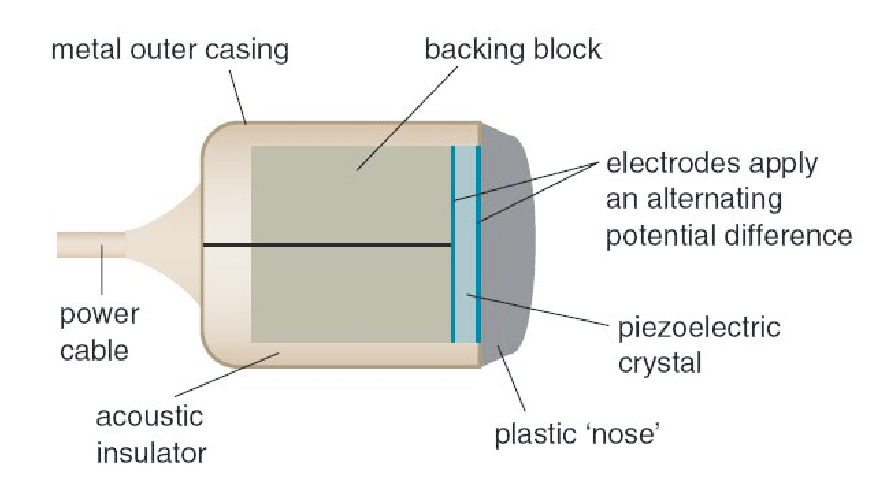
\includegraphics[width=0.7\textwidth]{UltrasoundTransducercollected.eps}\\
	\caption[Schematics of Ultrasound Transducer ]{Schematics of Ultrasound Transducer \footnote}\label{fig:Ultrasound transducer}
\end{figure}
\footnotetext{http://www.genesis.net.au/~ajs/projects/medical\_physics/ultrasound/index.html}

Figure ~\ref{fig:Ultrasound transducer} depicts a typical configuration of an ultrasound transducer. Its main component is a piezoelectric material\cite{Hendee.2003..317}.




\subsection{Piezoelectric Effect}
The phenomenon of piezoelectricity was first discovered by Jcques and Pierre Curie in 1880 where the observed that under the influence of mechanical stress certain crystal undergoes electrification. ~\cite{CurieP.1880.CRF.294}. Soon after that in 1881 a converse piezoelectric effect was derived mathematically by Lippman ~\cite{G.1881.AdCedP5s.145} using thermodynamic principles which was confirmed later by the curie brothers ~\cite{CurieP.1881.CRF.1137} on the same year. The latter effect was termed as indirect piezoelectric effect and the former one as direct piezoelectric effect. This phenomenon of piezoelectricity was observed only on certain materials like tourmaline,quartz,topaz,cane sugar and Rochelle salt mostly in the direction normal to polar axis. Based on this, it was concluded that this effect can be explained by the crystal symmetry study. Because of its unique nature, the discovery of piezoelectric materials created general interest among researchers  which led this material find use in underwater sonar, medical imaging instrument, car accelerometers etc.
\begin{figure}[t]
\centering
	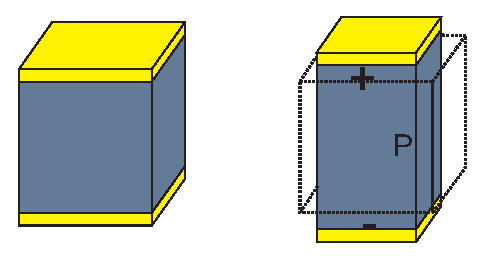
\includegraphics[width=0.7\textwidth]{Piezoelectric_final.eps}\\
	\caption[The Piezoelectric effect]{The Piezoelectric effect}\label{fig:The Piezoelectric effect}
\end{figure}
In a piezoelectric material under equilibrium condition, the electronic charge distribution of the constituent elements are balanced equally between positive and negative charges in order to make the crystal electrically neutral. When perturbation is applied in the means of mechanical stress (Direct piezoelectric effect), the equilibrium charge distribution is compromised by the mechanical strain. The strain produces lattice mismatch as a result the charge distribution are arranged in a way to produce a net resultant electrification in the material. This charge distribution characteristics are expressed by polarization. Similarly in a indirect or converse piezoelectric effect when electrified, the charge distribution is arranged in accordance to the direction and characteristics of applied electric field. To accommodate this charge perturbation a net resultant strain is generated inside the material.

\subsection{Ferroelectricity}
Several crystal class exhibits piezoelectric effect but ferroelectric materials due to their singular behavior of switching between two equilibrium states have drawn significant attentions. Ferroelectricity was discovered in 1917 while investigating the piezoelectric properties of Rochelle salt. It was observed that these materials shows anomalous dielectric behaviors like the existence of a hysteresis between applied electric field and polarization, sudden change in piezoelectric behavior under certain temperature condition.

\begin{figure}[t]
\centering
	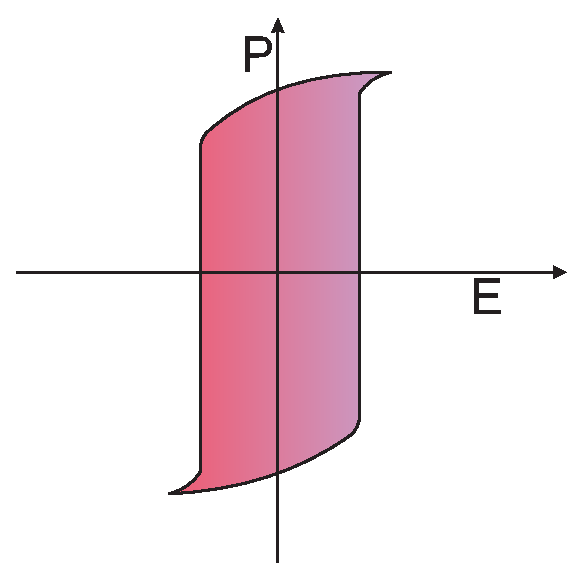
\includegraphics[width=0.4\textwidth]{Hysteresis.eps}\\
	\caption[The ferroelectric hysteresis]{The ferroelectric hysteresis}\label{fig:The ferroelectric hysteresis}
\end{figure}

A ferroelectric material is described as an insulting system having equivalent but opposite multiple states of non zero polarization in the absence of any electric field. This non zero polarization is defined as the spontaneous polarization. These multiple spontaneous polarization states are switchable among each other by application of an external electric field.Another interesting property that ferroelectric materials posses is their ability to inherit several stable structural phases. In most common cases, their structural arrangement holds an ferroelectric phase below a characteristic temperature called the curie temperature $T_{c}$. At the ferroelectric phase the material contains lower number of symmetry operation with the absence of inversion symmetry and as a result, the net charge distribution produces a polar distortions of the structure to generate a non zero spontaneous polarization. But as soon as the material exhibit temperature higher than the curie temperature the structure undergoes a transformation from ferroelectric to paraelectric phase. At this structural phase a higher degree of symmetry is present inside the structure which balances out the charge distribution to maintain a zero spontaneous polarization.

It is obvious that the charge distribution disruption which generates the spontaneous polarization is produced by change in atomic arrangement of ions from their symmetric positions. So the crystal must be polar in order to exhibit a ferroelectric behavior. However, not all the polar crystal have the ability to switch their polarization between two equivalent and opposite state (or the ability to switch between two equivalent atomic position). So in order to be considered as a ferroelectric, the crystal must also demonstrate the switching behavior which appears in situation when there is a symmetry breaking distortion from the higher symmetry state. Figure~\ref{fig:Two dimensional ferroelectric distortion}(a) shows 2 dimensional view of perovskite crystal in polar phase. At this stage the distribution of atoms is highly symmetric which also give rise to a symmetric charge distribution. Thus the net resultant charge inside the crystal cancel each other to give structure with zero polarization. On the other hand, in Figure~\ref{fig:Two dimensional ferroelectric distortion}(b) the movement of atoms from their equilibrium position lowers the symmetry  and the net charge distribution has a resultant in positive Z direction. The gives rise to a spontaneous polarization in that direction which confirms that the structure exists in a ferroelectric phase. Now, It is also evident from Figure~\ref{fig:Two dimensional ferroelectric distortion}(c) there is also an equivalent but opposite ferroelectric distortion is possible which gives to an equal spontaneous polarization in negative Z direction  which represents the equivalent but opposite ferroelectric state.
\begin{figure}[t]
\centering
	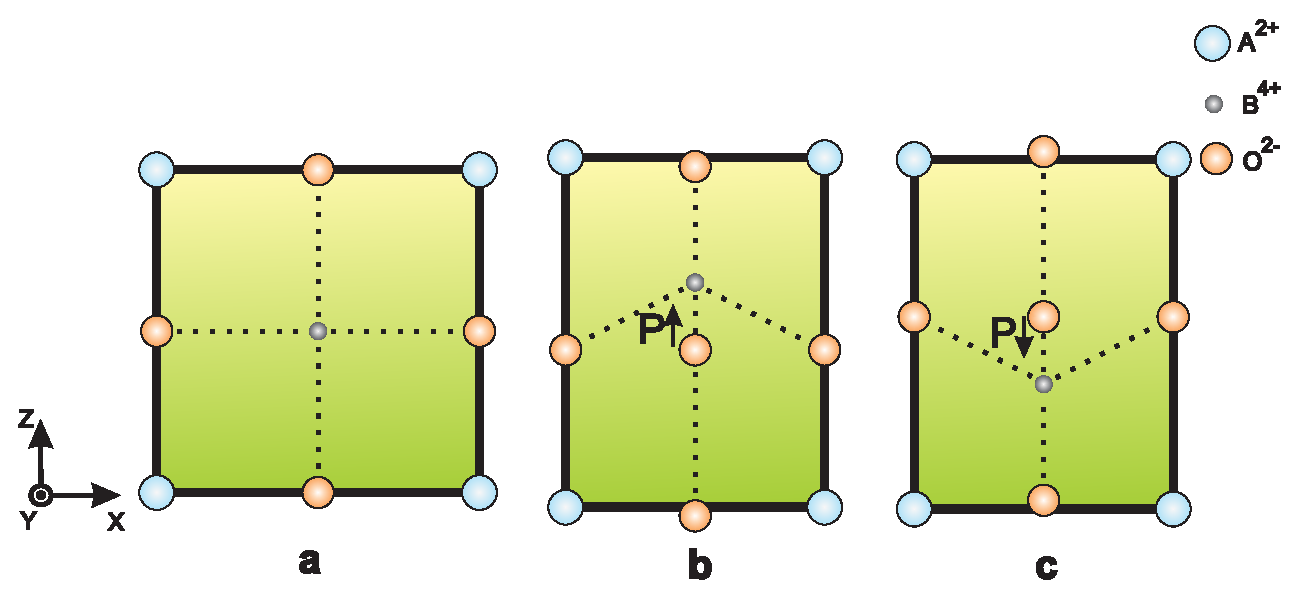
\includegraphics[width=1.0\textwidth]{Perovskite2D.eps}\\
	\caption[Two dimensional ferroelectric distortion]{Two dimensional ferroelectric distortion}\label{fig:Two dimensional ferroelectric distortion}
\end{figure}
\section{Current challenge in High Intensity Focused Ultrasound}
HIFU, despite of being one of the most promising treatment it is expensive. The majority of the high treatment cost comes from the involvement of MRI which costs about \$4000 per hour for a typical HIFU treatment.Beside the treatment also involves charges for surgeon and other miscellaneous costs. A typical HIFU operation time time is very long( more than $2-3$ hours).  which make a typical treatment cost of more than \$10000 for a 2 hours treatment.Also during the whole operation,the patient are restricted to move which causes discomfort to the patient. MRI involvement during the treatment is essential as it monitors the thermal ablation process. But, the longer operation time which is responsible for the higher treatment cost comes because of a delay in sonication heating pulse. Figure ~\ref{fig:Heating and Cooling pulse in HIFU treatment} depict a typical heating and delay cycle applied during HIFU operation which suggests the time utilization efficiency of around $30$\%.\begin{figure}[t]
\centering
	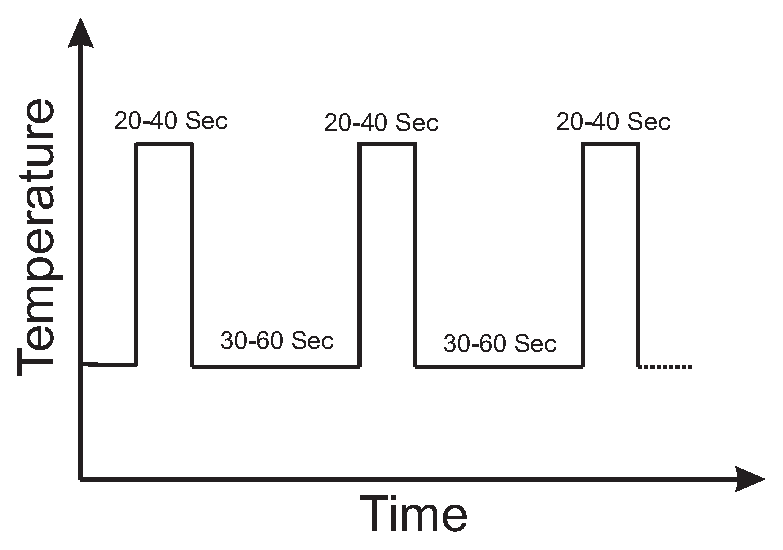
\includegraphics[width=0.7\textwidth]{HeatingandCoolingpulse.eps}\\
	\caption[Heating and delay cycle in HIFU treatment]{Heating and delay cycle in HIFU treatment}\label{fig:Heating and Cooling pulse in HIFU treatment}
\end{figure} This longer delay in sonication is applied in order to prevent thermal build up due to cumulative build up of ultrasound  near the transducer[Add reference]. This thermal build up if not prevented, can result in bubble because of boiling of water in the nearby tissue. Because of these bubble the focused ultrasound beam can get reflected or scattered near the bubble originating places places which in turn can results in deviation of path of the focused ultrasound.[Add reference]. Also from the transducer point of view, sufficient thermal build up can the expansion of the ferroelectric materials which will lead to the violation of  effective thickness-resonance frequency relationship (Equation~\ref{Eq:Effectivethichness-frequency})  and as a result dampening of ultrasound. And in worst case scenario, too much thermal build up can cause depolarization of the ferroelectric material if the temperature is near the curie temperature of the material. Besides during the sonication this thermal build up causes much discomfort to the patient.

\subsection{Factor to focus: Dielectric dissipation factor, Hysteresis}
Thermal build up is resulted due to overheating of the ferroelectric materials during sonication and this is  dependant on the ferroelectric material itself. The associated material characteristic is called dielectric dissipation factor, tan$\delta$.
Dielectric dissipation factor is a measure of parasitic loss that results by subjecting a material to alternating electric field. \begin{figure}[t]
\centering
	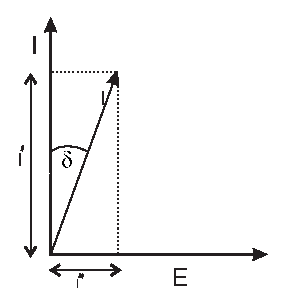
\includegraphics[width=0.7\textwidth]{E-Icharacteristics.eps}\\
	\caption[Loss current in a dielectric]{Loss current in a dielectric}\label{fig:Loss current in a dielectric}
\end{figure}As shown in figure ~\ref{fig:Loss current in a dielectric} when an electric field, E is applied in an ideal material the resultant charging current find itself out phase by $90^{0}$ with the applied electric field. But in a typical ferroelectric material which is essentially a dielectric the current also has an loss component in phase with applied electric field and the net resultant current makes an angle $\delta$ with the ideal charging current. This loss current is a result of dissipation of energy as heat. This loss can interpreted using the parameter tan$\delta$ which is the ratio of loss current and charging current.
 \begin{equation}\label{Eq:tandeltacurrentloss}
    tan\delta =\frac{Loss\ Current,I"}{Charging\ Current, I'}
\end{equation}
Now,the current flowing throw the material is related to the capacitance(C), applied electric field(E), frequency of the applied electric field($\omega$) and the dielectric constant of the material($\varepsilon$) in the following way,
 \begin{equation}\label{Eq:currentand capacitance}
    I=E\omega\varepsilon C
\end{equation}

So the dielectric dissipation factor can also be express as a ratio of the complex part of the dielectric constant and real part of the dielectric constant.
\begin{equation}\label{Eq:tandeltacurrentloss}
    tan\delta =\frac{\varepsilon"}{\varepsilon'}
\end{equation} 

The reason that there is a loss component is that during the application of alternating electric field to ferroelectric materials the polarization doesn't get enough time to attain equilibrium with the applied field. This lag is due to the fact that the  forces in the system can't change according to the which it is subjected. Normally, in a process involve application of alternating current to a ferroelectric materials during ultrasound generation involves application of frequency in  MHz range which means it gets time of around $1e^{-6}$ seconds. But as polarization requires much more time in order to attain equilibrium with applied electric field, this generates a lag between applied electric field and polarization.Mathematically, the applied alternating electric field has the following form,
\begin{equation}\label{Eq:Elelctricfield}
    E =E_{0}e^{i\omega t}
\end{equation}
Because of the lag in response the polarization has the following form,
  \begin{equation}\label{Eq:Polarization}
    P =P_{0}e^{i\omega t-\delta}
\end{equation}
As a result of this delay, the polarization Vs electric field curve takes an hysteresis form. 

\begin{figure}[t]
\centering
	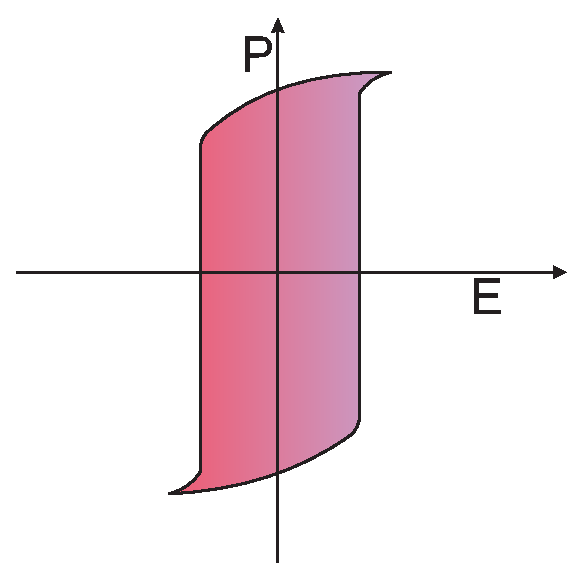
\includegraphics[width=0.4\textwidth]{Hysteresis.eps}\\
	\caption[The ferroelectric hysteresis]{The ferroelectric hysteresis}\label{fig:The ferroelectric hysteresis}
\end{figure}
\chapter{Figures and Tables}
\label{chap:figtab}

\section{Figures}

We can include encapsulated PostScript\texttrademark\ figures
(\texttt{.eps}) in the document and refer to it using a label.
For example, MUN's logo can be seen in Figure~\ref{fig:MUN_Logo_Pantone}.
\munepsfig{MUN_Logo_Pantone}{This is MUN's logo}

Figure~\ref{fig:enrollment} shows a chart of MUN's Fall
enrollment from 2005 -- 2009.\munfootnote{From \emph{Memorial
University of Newfoundland --- Fact Book 2009}.}
\munepsfig[scale=0.50]{enrollment}{MUN Fall Enrollment 2005 -- 2009}
The figure was created using the \textsf{Calc} spreadsheet application of
the office suite \textsf{OpenOffice.org}.\munfootnote{This office suite
can be downloaded at no cost from \texttt{http://openoffice.org/}. Unlike
other commercial office suites, \textsf{OpenOffice.org} may be legally
shared with colleagues and fellow students.  There are versions for
Linux, Microsoft Windows, Mac~OS~X and Solaris.  Also, unlike commercial
offerings, \textsf{OpenOffice.org} does not require activation using
registration keys.}  This figure was reduced by 50\%.

For larger figures, we can use landscape mode to rotate the page
and display the figure using the \verb+\munlepsfig+ command, as shown
in Figure~\ref{fig:enrollment-landscape}.  The figure will be the
only thing on the page when typeset in landscape mode. 
(The figure is reduced to 85\% of its original size.)
\munlepsfig[scale=0.85]{enrollment-landscape}
	{MUN Fall Enrollment 2005 -- 2009 (landscape)}

Alternatively, if we just want to rotate the figure, but not 
the entire page, we can specify an \texttt{angle} attribute
in the default argument of the \verb+\munepsfig+ command.
The result is shown in Figure~\ref{fig:enrollment-rotate}.
If the figure is too large or if there isn't sufficient
text, then the figure may appear on its own page.
\munepsfig[scale=0.30,angle=90]{enrollment-rotate}
	{MUN Fall Enrollment 2005 -- 2009 (rotated)}

Note that all three of the enrollment figures are basically
the same file, but with different names --- on Linux, they are
symbolic links to the same file.  The filenames have to be different
because the reference labels need to be unique.

Figure~\ref{fig:db-deadlock} shows a Petri net created using the
\texttt{xfig} program (\texttt{http://www.xfig.org/}) which has
very good support for \LaTeX.  This figure has been
reduced to 40\% of its original size.
\munepsfig[scale=0.40]{db-deadlock}{A deadlocked Petri net}

We can also create figures of text (such as short code snippets)
using the \verb+\muntxtfig+ command, as show in Figure~\ref{fig:code}.
\begin{muntxtfig}[1.0]{code}{Hello World}{0.5\textwidth}
\begin{verbatim}
#include <stdio.h>

int main(int argc, char **argv)
{
  printf("Hello world!\n");
  exit(0);
}
\end{verbatim}
\end{muntxtfig}

\section{Tables}

We can also create tables, as seen by Table~\ref{tab:pop}.  Note that,
as required by SGS guidelines, the caption for a table appears above the
table whereas figure captions appear below the figures.  Tables and
figures can ``float'' --- they may not appear on the page on which they
are mentioned.  \LaTeX{} tries to handle figure and table placement
intelligently, but if if you have a lot of them without a reasonable
amount of surrounding textual content, the figures and tables can
accumulate towards the end of the chapter.  Generally speaking, if
there is sufficient text explaining the tables and figures or if the
tables/figures are relatively small, this may not be a problem.  However,
if you have a lot of tables or figures, it may be a good idea to put
them in an appendix and refer to them as the need arises.

\begin{muntab}{c||c|c|c||c|c|c|}{pop}{Fall Semester Enrollment}
\hline
	& \multicolumn{3}{c||}{Undergraduate}
	& \multicolumn{3}{c|}{Graduate} \\
\cline{2-7}
     & F/T & P/T & Total & F/T & P/T & Total \\
\cline{2-7}
2004 & 13,191 & 2,223 & 15,414 & 1,308 & 879 & 2,187 \\
2005 & 13,184 & 2,143 & 15,327 & 1,375 & 920 & 2,295 \\
2006 & 12,809 & 2,224 & 15,033 & 1,373 & 899 & 2,272 \\
2007 & 12,634 & 2,155 & 14,789 & 1,403 & 899 & 2,302 \\
2008 & 12,269 & 2,208 & 14,477 & 1,410 &1,005& 2,415 \\
2009 & 12,382 & 2,323 & 14,705 & 1,567 &1,106& 2,673 \\
\hline
\end{muntab}

Table~\ref{tab:degrees} shows a different table in landscape
mode.\munfootnote{This data was also taken from the \emph{Memorial
University of Newfoundland --- Fact Book 2009}.} This is useful if your
table is too wide for the page.  Tables are double-spaced by default.
To single-space a table, change the \verb+\baselinestretch+ before
beginning the table environment.  Remember to restore it after the
environment has ended.

\renewcommand{\baselinestretch}{1.0}\normalsize
\begin{munltab}{lrrrrrrrrrrrr}
	{degrees}
	{Masters Degrees Conferred by Convocation Session --- 1950 to 2009}
\cline{2-13}
				&
\multicolumn{2}{|c|}{2009}	&
\multicolumn{2}{c|}{2008}	& 
\multicolumn{2}{c|}{2007}	& 
\multicolumn{2}{c|}{2006}	& 
\multicolumn{2}{c|}{2006}	& 
\multicolumn{1}{c|}{1950--2004}	& 
\multicolumn{1}{c|}{Total}	\\
\cline{2-13}
	  &
May & Oct &
May & Oct &
May & Oct &
May & Oct &
May & Oct & &  \\
Degrees \\
\hline
Master of Applied Science		&  14 &   2 &  15 &   8 &  28 &   1 &  21 &   3 &   3 &   1 &    98 &   194 \\
Master of Applied Social Psychology     &   1 &   5 &   2 &   5 &   1 &   4 &   0 &   4 &   0 &   4 &    28 &    54 \\
Master of Applied Statistics            &   0 &   0 &   3 &   1 &   0 &   0 &   1 &   0 &   0 &   0 &    19 &    24 \\
Master of Arts                          &  37 &  49 &  26 &  43 &  14 &  42 &  14 &  56 &  13 &  44 &   994 & 1,332 \\
Master of Business Administration       &  14 &  16 &  23 &   6 &  33 &  12 &  33 &  11 &  33 &   8 &   818 & 1,007 \\
Master of Education                     & 107 &  87 & 120 &  55 & 147 &  74 & 108 &  76 & 113 &  75 & 2,603 & 3,565 \\
Master of Employment Relations          &   8 &   9 &   5 &   7 &   7 &  14 &   4 &   9 &   3 &   5 &    12 &    83 \\
Master of Engineering                   &  20 &  19 &  20 &  10 &  16 &  10 &  15 &  13 &   4 &  19 &   440 &   586 \\
Master of Environmental Science         &   3 &   3 &   3 &   1 &   0 &   1 &   7 &   1 &   3 &   1 &    66 &    89 \\
Master of Marine Studies                &   2 &   0 &   0 &   1 &   0 &   2 &   2 &   2 &   1 &   2 &    26 &    38 \\
Master of Music                         &   4 &   1 &   5 &   0 &   3 &   0 &   3 &   0 &   3 &   0 &     7 &    26 \\
Master of Nursing                       &   7 &   8 &  10 &   4 &  17 &   4 &  23 &   7 &   6 &   1 &   116 &   203 \\
Master of Oil and Gas Studies           &   0 &   0 &   2 &   0 &   0 &   0 &   0 &   2 &   4 &   0 &     0 &     8 \\
Master of Philosophy                    &   5 &   4 &   2 &   1 &   5 &   2 &   5 &   3 &   2 &   0 &   112 &   141 \\
Master of Physical Education            &   0 &   2 &   3 &   0 &   5 &   4 &   3 &   0 &   4 &   4 &    84 &   109 \\
Master of Public Health                 &   0 &   8 &   0 &   0 &   0 &   0 &   0 &   0 &   0 &   0 &     0 &     8 \\
Master of Science                       &  40 &  32 &  41 &  19 &  29 &  25 &  35 &  29 &  32 &  23 & 1,653 & 1,958 \\
Master of Science (Kinesiology)         &   1 &   0 &   4 &   2 &   1 &   2 &   2 &   6 &   4 &   3 &     0 &    25 \\
Master of Science (Medicine)            &  18 &   7 &  11 &   8 &  10 &   5 &   9 &   9 &   8 &   4 &     0 &    89 \\
Master of Science (Pharmacy)            &   0 &   0 &   1 &   1 &   0 &   0 &   0 &   0 &   1 &   0 &    16 &    19 \\
Master of Social Work                   &   4 &  11 &   4 &   5 &   4 &   9 &   9 &   5 &   4 &  10 &   257 &   322 \\
Master of Women's Studies               &   2 &   0 &   2 &   0 &   1 &   1 &   2 &   3 &   2 &   0 &    20 &    33 \\
\hline
\textbf{Total Masters}                  & 287 & 263 & 302 & 177 & 321 & 212 & 296 & 239 & 243 & 204 & 7,369 & 9,913 \\
\end{munltab}
\renewcommand{\baselinestretch}{\spacing}\normalsize

\chapter{Dealing with Errors}
\label{chap:errors}

\LaTeX{} can produce cryptic error messages at times.
However, with some experience, it is usually not too
difficult to determine what the problem is and how to fix it.

As mentioned earlier, appropriate search terms in Google
may help you fix these error messages.


\chapter{Lorem Ipsum}
\label{chap:ch4_abbr}
Now, for your reading pleasure, some \textsl{Lorem ipsum}, courtesy
of:
\begin{center}
\texttt{<http://www.lipsum.com/>}
\end{center}
This gives a good view of the margins --- note that the left margin
is a bit wider than the right margin to accommodate binding.

Lorem ipsum dolor sit amet, consectetur adipiscing elit. Etiam odio elit,
viverra eu tempor non, pulvinar ac nisi. Pellentesque habitant morbi
tristique senectus et netus et malesuada fames ac turpis egestas. Sed
adipiscing, dui quis viverra facilisis, quam libero adipiscing justo,
vitae dictum libero mauris ac magna. Aenean sem ligula, vulputate at
vestibulum eu, pellentesque in justo. Sed et eros mauris, sed placerat
nulla. Maecenas nulla velit, facilisis et rutrum nec, volutpat id
lorem. Duis vestibulum odio velit, id elementum tortor. Sed pellentesque
leo ac nibh iaculis at fermentum orci lobortis. Suspendisse arcu magna,
porta nec pretium non, feugiat vitae orci. Vivamus at enim arcu,
at sagittis nisl. Vestibulum at mi enim, vel malesuada justo. Class
aptent taciti sociosqu ad litora torquent per conubia nostra, per
inceptos himenaeos. Nullam sed nunc at enim posuere sagittis. Vivamus
augue turpis, mattis a blandit non, sollicitudin non nisl. Integer
vestibulum, est vitae cursus adipiscing, elit libero pretium leo,
in scelerisque augue felis volutpat nisl. Donec commodo posuere arcu,
eget feugiat dui ornare nec. Nullam eros mi, condimentum ac ultricies ac,
euismod lobortis nibh. Cras ac ligula pharetra risus elementum pharetra
vel in quam. Fusce ac augue vulputate nibh imperdiet convallis sit amet
et quam. Integer porttitor dictum fermentum.

Nullam id ante arcu. Nulla facilisi. Vestibulum sodales, mi sodales
ultricies pulvinar, orci leo dictum diam, quis imperdiet turpis lacus
ut sem. Nulla rutrum odio sit amet elit aliquam blandit gravida nunc
placerat. Aenean et neque ut leo condimentum vehicula. Fusce quis orci
vitae enim dapibus tincidunt in vel ipsum. Phasellus auctor neque ac eros
egestas sit amet ultricies erat vestibulum. Ut erat ligula, pharetra
vel hendrerit vitae, mattis ac turpis. Ut malesuada diam vitae lacus
vestibulum a tempus nisl posuere. Ut nisi sem, dictum eu laoreet sed,
commodo eget enim. Morbi vel lacus neque, tempus fringilla tellus. Nunc
id egestas felis. Nullam eu mollis neque. Ut non mauris malesuada
eros sagittis congue. Cras vitae felis ut nisl mollis semper ut quis
risus. Sed eu arcu urna, et commodo sapien. Donec vestibulum, libero
sit amet ultrices blandit, erat lorem volutpat lectus, sed feugiat leo
elit in orci. Aliquam vitae leo tellus, placerat pulvinar massa. Nulla
at sapien hendrerit diam varius vehicula.

Curabitur et orci nulla. Phasellus euismod, massa non hendrerit dictum,
dolor enim imperdiet sapien, vitae commodo lorem tellus eu quam. Duis
egestas felis velit. Sed in orci nec nulla rutrum posuere. Suspendisse
potenti. Nunc vel quam nisi. In at molestie libero. Aenean hendrerit
vestibulum orci, ut hendrerit nulla volutpat lacinia. Vestibulum sit amet
sapien vitae lectus gravida vehicula. Suspendisse ac purus sit amet est
congue auctor.

Morbi pellentesque, quam vel mattis molestie, augue purus vestibulum
lorem, nec consequat enim eros eu augue. In odio dolor, scelerisque
a lobortis porttitor, commodo ut lacus. Maecenas sit amet diam
nec tellus accumsan bibendum. Praesent in turpis velit, malesuada
commodo sapien. Nunc ornare urna enim. Sed at diam non metus porttitor
suscipit. Aliquam erat volutpat. Duis aliquet magna in mauris semper
placerat. Ut eget quam orci. Ut egestas, dolor at dapibus accumsan, leo
nibh egestas urna, ac consectetur dui odio quis eros. Nam libero dolor,
lacinia eget imperdiet non, malesuada vehicula diam. Etiam id ipsum eget
turpis consectetur tristique id at ante. Vivamus blandit nunc eu nisl
varius sed accumsan odio molestie.


\chapter{Handling Citations}
\label{chap:refs}


\chapter{Conclusions}
\label{chap:conclusions}
That's all folks!


\addcontentsline{toc}{chapter}{Bibliography}
\bibliographystyle{ieeetr}
\bibliography{library} 
\expandafter\ifx\csname natexlab\endcsname\relax\def\natexlab#1{#1}\fi
\expandafter\ifx\csname bibnamefont\endcsname\relax
  \def\bibnamefont#1{#1}\fi
\expandafter\ifx\csname bibfnamefont\endcsname\relax
  \def\bibfnamefont#1{#1}\fi
\expandafter\ifx\csname citenamefont\endcsname\relax
  \def\citenamefont#1{#1}\fi
\expandafter\ifx\csname url\endcsname\relax
  \def\url#1{\texttt{#1}}\fi
\expandafter\ifx\csname urlprefix\endcsname\relax\def\urlprefix{URL }\fi
\providecommand{\bibinfo}[2]{#2}
\providecommand{\eprint}[2][]{\url{#2}}


% If you have no appendices, remove the following two lines.
% If you have more appdences, add them as necessary.
\appendix
\chapter{Appendix title}
\label{apdx:somelabel}
This is Appendix~\ref{apdx:somelabel}.

You can have additional appendices too
(\emph{e.g.}, \texttt{apdxb.tex}, \texttt{apdxc.tex}, \emph{etc.}).
If you don't need any appendices, delete the appendix
related lines from \texttt{thesis.tex} and the file names
from \texttt{Makefile}.


\end{document}
